\documentclass[11pt]{article}
\usepackage{evolution}

\begin{document}

%--------------------------------------------------
% Titlepage
%--------------------------------------------------

\begin{center}
    \textbf{When your favorite trait is not enough to explain diversification: An example of diversification linked to polyploidy and breeding system in Solanaceae}
\end{center}

\vfill

\noindent
Rosana Zenil-Ferguson,%
\endnote{University of Minnesota Twin Cities}
%
\noindent
J. Gordon Burleigh,%
\endnote{University of Florida}
%
\noindent
William A. Freyman,%
\endnote{23 and me}
%
\noindent
Boris Igi\'c,%
\endnote{University of Illinois}
%
\noindent
Itay Mayrose,%
\endnote{Tel Aviv University}
%
and
Emma E. Goldberg%
\endnote{University of Minnesota Twin Cities}

\vfill

\theendnotes

\noindent
Author for correspondence: Rosana Zenil-Ferguson

\vfill

\noindent
\textit{Running head:} Polyploidy and breeding systems in Solanaceae

\vfill

\noindent
\textit{Keywords:} 
Polyploidy,
Breeding System,
Diversification, SSE models

\vfill

\linenumbers

%--------------------------------------------------
% Abstract
%--------------------------------------------------

\clearpage
\section{Abstract}

Abstract text\ldots


%--------------------------------------------------
% Main text
%--------------------------------------------------

\clearpage
\section{Introduction}


% Outline, discussed by Boris and Emma:
%
% we are interested in the evolution of traits and their influence on lineage diversification
%     ref Barrett work 
% 		no diversification?, but trait shifts:
%		barrett_1996 (mating system + LH)
%		barrett_2013
%		barrett_2008: "Because polyploidy affects the entire genome, it is perhaps not surprising that it influences many as- pects of the phenotype, including the mating system. However, although it has long been recognized that the evolutionary tran sition from diploidy to polyploidy may result in correlated changes in mating patterns, the theoretical and empirical evidence is limited and often contradictory." (p.5)
%
%     any one study focuses on one/few traits
%     but any real organisms have many, so need to enlarge our view
%     mini "here, we..."
% we have tools to try to answer these questions
%     sse models
%     issues
%     but a way forward is to allow for multiple factors that could influence diversification
% ploidy
%     Stebbins
%     Mayrose, Soltis
%     recent paleo WGD, diploidization
% breeding system
%     directionality
%     diversification in Solanaceae
%     correlation with ploidy
%     pathways from SI-D to SC-P: direct or via SC-D
% here, we...
%     diversification: interaction between ploidy and breeding system
%     also: diploidization, pathways

%B: I placed this out of order, so you can see it
The prevalence and significance of polyploidy was broadly considered a salient feature of flowering plants \citep{}, even before the advent of genomic tools dramatically escalated the stakes, so that nearly flowering plants are thought to have undergone at least one round of polyploidization \citep{}.
It is therefore perhaps surprising that there appears to be little agreement regarding the evolutionary consequences of polyploidy, especially how it affects diversification rates. %species richness.
% I think Rosana wants this part here (above)
% next, continue with ploidy narrative (mayrose/soltis)

Polyploidization changes the genomic content of all cells, and consequently has the potential to affect a wide variety, if not all, traits. 
Among the many of changes associated with polyploidization, perhaps the most prominent is the association between polyploidy and propensity for self-fertilization \citep{stebbins1950, barrett1988}.
Polyploidy is not only a suspected correlate of breeding systems but a causal link \citep{stout1942, lewis1947}.
Doubled number of alleles in pollen is strongly suspected to effect disruption of the genetic mechanisms in gametophytic self-incompatibility systems \citep{entani1999, tsukamoto2005, kubo2010}. 
Polyploidy is also thought to be associated with changes in the rate of self-fertilization, although the evidence for this correlated shift in mating system appears limited and sometimes contradictory \citep{barringer2007, barrett2008, husband2008}.
% It's not Spencer's best line, but it's not bad for our work: Barrett 2008: "Because polyploidy affects the entire genome, it is perhaps not surprising that it influences many aspects of the phenotype, including the mating system. However, although it has long been recognized that the evolutionary transition from diploidy to polyploidy may result in correlated changes in mating patterns, the theoretical and empirical evidence is limited and often contradictory."
% how that generates associations (and variable associations of mating system and ploidy! husband2008, others cited by barrett2013
Breeding system shifts---changes in the collection of physiological and morphological traits that determine the likelihood that any two gametes unite---are remarkably common and affect the distribution and amount of genetic variation in populations \citep{stebbins1974,barrett2013}.
They are by themselves thought to have a broad effect on other traits. 
The frequent transition from self-incompatibility (SI) to self-compatibility (SC) is strongly associated with net diversification rate changes \citep{goldberg_2010,devos2014}.
Given that  changes in ploidy and breeding systems may be causally related and have profound profound affects on the fate of lineages, it seems particularly profitable to examine whether and how their macroevolutionary effects interact.
%
% we also have this great data for SI loci and the transition could be even more common, providing power to resolve the great diversification questions
%
% set up pathway dependence


Studying diversification linked to trait evolution\newline
% Here I need help (perhaps will be the last line I write)
%In these context, botanist have been asking how polyploidy shapes patterns of diversification. 
The prevalence of polyploidy and its detection across multiple and highly diverse clades of angiosperms inevitably lead to the hypothesis of the importance of polyploidy in the speciation and extinction patterns observed across the flowering plant phylogeny. 
At the same time, a similar question has been asked in the breeding system world, where self-compatibility has evolved multiple times in flowering plants. 
However, the influence in diversification using both polyploidy and self-compatibility information has not been studied simultaneously.

- Why polyploidy and self-compatibility in particular makes for an  interesting study in the context of diversification\newline
In the polyploidy world, an important debate regarding the diversification of angiosperms has been ongoing since the publication of \citet{mayrose_2011}. The authors discovered that using the latest diversification model linked to two states diploid and polyploid, the net diversification of polyploids was much slower than the net diversification rate than polyploids. This result was surprising and an sparked a discussion about the long-term evolutionary consequences of polyploidy. \citet{soltis_2014} questioned if polyploidy should be regarded as an evolutionary dead-end since the net diversification of polyploids was negative, despite overwhelming evidence about the incidence of polyploidy  especially at the root of highly diverse angiosperm claims (ref here). A year later, diversification models were re-tested and corrected, and still found the same pattern \citep{mayrose_2015}, to the disappointment of plenty of botanists there was no denying of the weak trend of diversification that polyploids left behind. The most recent study by \citet{landis_2018} that used not only the presence of polyploidy in the tips but also the number of whole genome duplications in a taxon lineage found that.... \newline  Meanwhile, studies focusing on diversification patterns and  breeding system have consistently found that self-incompatible plants often have higher net diversification rates compare to their self-compatible counterparts (Emma and Boris' papers here, what about papers that are not solanaceae?) 

- Why other traits need to be considered as well\newline


- What other models and studies have done in the past\newline

- What is lacking from past approaches? \newline
There are two key questions that at the time of the polyploidy debate were difficult to ask. The first is if the models used to measure the diversification of polyploids were correct, and the second question is if the models have potentially included more evidence and potential traits that are not polyploidy or other lines of evidence that could be driving the patterns. At the time, in a different context \citet{beaulieu_2016} were finding an alternative solution to the first question, coming up with a new model that could represent the broad heterogeneity of the diversification process and parse out the signal between the trait of interest and the noise in diversification. Their model, the hidden state speciation and extinction model is a key component to detect whether polyploidy our something else unknown but related to it is driving the speciation and extinction patterns that we see in angiosperms. \newline
What is our proposal to tackle this problem?\newline

The second question (talk here about breeding system and polyploidy, and how this could be different across clades and this is one of the reasons why we focused on Solanaceae).
-Diversification and breeding systems\\
Goldberg and Igic 2012, different  perspectives\\

\section{Methods}

\subsection{Data}

%B: IMO: The data subsection would be better organized with parts, (1) ploidy, (2) breeding system, (3) tree, (4) models, (5) model selection and statistical inference.

Chromosome number data were obtained for all Solanaceae taxa in the Chromosome Counts Database \citep[CCDB;][]{rice_2015}, and the ca.~14,000 records were curated semi-automatically using the CCDBcurator R package \citep{rivero_2019}. CCDB contains records from original sources that have multiple complex symbol patterns denoting multivalence, or irregularites of chromosome counts. After a first full round of curation via CCDBcurator, we contrasted results by hand and corrected chromosomes where CCDBcurator's output was not able to curate.  Our hand curated records were also contrasted against the large dataset Solanaceae ploidy states from \citet{robertson_2011} and against ploidy data from the C-value DNA dataset from Kew royal botanic gardens \citep{bennett_2005}.
  %B: perhaps "cleaned" should be explained, unless it's hard to identically repeat as-is. R- I added more (it only took 4months to hand-curate 14,000 entries
By contrasting three sources of information, we were able to code taxa as diploid (D) or polyploid (P).
For the majority of species, ploidy was assigned according to information from the original publications and the Kew royal botanic gardens C-value DNA resource \citep{bennett_2005}.
For taxa without ploidy information but with information about chromosome number, we assigned ploidy based on the multiplicity of chromosomes within the genus or based on information of incompatibility. If a species was incompatible without any chromosomal information it was assigned as diploid.
For example, \textit{Solanum betaceum} did not include information about ploidy level but it has 24 chromosomes, since $x=12$ is the base chromosome number of the \textit{Solanum} genus \citep{olmstead_2007}, we assigned \textit{S.~betaceum} as diploid. 
Species with more than one ploidy level were assigned the smallest of most frequent ploidy level recorded.
% E: There was more here about cross-verifying that no P species were SI.  I removed it because there were conflicts before, but we resolved them.  This is addressed in the next paragraph.
%
Breeding system was scored as self-incompatible (I) or self-compatible (C) based on results curated from the literature and  original experimental crosses \citep[as compiled in][]{igic_2006, goldberg_2010, robertson_2011, goldberg_2012}.
Most species could unambiguously be coded as either I or C \citep{raduski_2012}.  But for diploids without breeding system information taxa was coded as both I or C.%B: most? Any exceptions?
Following previous work, we coded as I any species with functional I systems, even if C or dioecy was also reported.
Dioecious species without functional I were coded as C.

% E: I am trying to stick with I/C when talking about the state values, but using SI/SC when talking about the meaning of the trait (because this what people use normally).

To those existing data sets, we added some additional records for chromosome number and breeding system.
The Supplementary Information contains citations for the numerous sources for the added data. % todo: add number of refs when we have it
Resolution of taxonomic synonymy followed the conventions provided in Solanaceae Source \citep{solsource}. 
Hybrids and cultivars were excluded because ploidy and breeding system can be affected by artificial selection during domestication.
Following the reasoning outlined in \citet{robertson_2011}, we examined closely the few species for which the merged ploidy and breeding system data indicated the presence of self-incompatible polyploids.
Although I populations frequently contain some C individuals, and diploid populations frequently contain some polyploid individuals, in no case did we find a convincing case of a naturally occurring I and polyploid population.
%B: Thus qualified, as above, I think this should be inserted.
The single instance of an I and polyploid individual appears to be an allopentaploid hybrid of {\em Solanum oplocense} Hawkes x {\em Solanum gourlayii} Hawkes, reported by \citealt{camadro_1981}.
Under exceedingly rare circumstances, it is possible for polyploids containing multiple copies of S-loci to remain I, so long as they express a single allele at the S-locus (discussed in \citealt{robertson_2011}).
Because of the resulting absence of I and polyploid populations, as well as the linked functional explanation for disabling of gametophytic self-incompatibility systems with non-self recognition, following whole genome duplication \citep[reviewed in][]{ramsey_1998,stone_2002}, we consider only three observed character states: self-incompatible diploids (ID), self-compatible diploids (CD), and polyploids which are always self-compatible (CP).
%B: I added the non-self recognition bit, because in Prunus, heteroallelic pollen may not cause SC.
% E: Should we include more details about how many polymorphic species and how the particularly tricky ones were dealt with? %B: No and yes, maybe.

Matching our character state data to the largest time-calibrated phylogeny of Solanaceae \citep{sarkinen_2013} yielded 595 species with ploidy and/or breeding system information on the tree.
Binary or three-state classification of ploidy and breeding system for the 595 taxa is summarized in \cref{figure:stateclassifications}.
We retained all of these species in each of the analyses below because pruning away tips lacking breeding system in the ploidy-only analyses (and vice versa) would discard data that could inform the diversification models.
A total of 405 taxa without any information about breeding system or polyploidy were excluded.
Tips without trait data are much less informative for diversification parameters linked to trait values.
Including this many more species would have prohibitively slowed our analyses, especially those implementing the most complex models.

% D/P ploidy model
% D/P+A/B ploidy hidden state model
% I/C breeding system model
% I/C+A/B breeding system and hidden state model
% ID/CD/CP ploidy and breeding system model
% ID/CD/CP+A/B ploidy, breeding system, and hidden state model

% NOTE: Should subtly rephrase so that the default models lack diploidization.

\subsection{Models for ploidy and diversification}

To investigate the association between ploidy level and diversification, we first defined a binary state speciation and extinction model (BiSSE, \citealt{maddison_2007}) in which taxa were classified as diploid (D) or polyploid (P) (\cref{figure:stateclassifications}).
We call this the \textit{D/P ploidy} model. %B: emphasis on introduced term (quotes awkward)
In a Bayesian framework, we obtained posterior probability distributions of speciation rates ($\lambda_D$, $\lambda_P$), extinction rates ($\mu_D$, $\mu_P$), net diversification rates ($r_D=\lambda_D-\mu_D$, $r_P=\lambda_P-\mu_P$), and relative extinction rates ($\nu_D=\mu_D / \lambda_D$, $\nu_D=\mu_D / \lambda_D$) associated with each state.
This analysis explores the same question as \citet{mayrose_2011, mayrose_2015}, using the polyploidization (parameter $\rho$, the transition rate from $D$ to $P$). % E: presumably the motivation will be explained in the Intro
%B: should the term above be "re-diploidization" or "diploidization" (as now)?

% B (via E): need some explanation of what \delta means, biologically, when ploidy is scored like this

Our second model assesses the signal of diversification due to ploidy differences while also parsing out the heterogeneity of diversification rates due a possible unobserved trait.
BiSSE-like models can suffer from a large false discovery rate because they fail to account for diversification rate changes that do not directly depend on the trait of interest \citep{rabosky_2015, beaulieu_2016}.
Diversification rate differences explained by some trait other than ploidy, are accommodated by adding a hidden state (HiSSE model; \citealt{beaulieu_2016}). %B: inserted "(trait)", because that seems to be the goal - a biological explanation?
In this model, each of the observed diploid and polyploid states is subdivided by a binary hidden trait with states $A$ and $B$.
We call this the \textit{D/P+A/B ploidy and hidden state} model. 
We estimated the posterior probability distributions of speciation rates ($\lambda_{D_A},\ \lambda_{D_B},\ \lambda_{P_A},\ \lambda_{P_B}$), extinction rates ($\mu_{D_A},\ \mu_{D_B},\ \mu_{P_A},\ \mu_{P_B}$), net diversification rates ($r_{D_A},\ r_{D_B},\ r_{P_A},\ r_{P_B}$), and relative extinction rates ($\nu_{D_A},\ \nu_{D_B},\ \nu_{P_A},\ \nu_{P_B}$).
In this model polyploidization rate  is again represented by $\rho$  and hidden states are symmetrical with rate $\alpha$. %B: same dip vs. re-dip question, as above.

\subsection{Models for breeding system and diversification}

To assess the effects of breeding system in the diversification process, we first fit model in which the states are self-incompatible (I) or self-compatible (C).
This is the same as the analysis of \citet{goldberg_2010}, save for an updated phylogeny \citep{sarkinen_2013}.
We call this BiSSE model the \textit{I/C breeding system} model. 
To parse out the effect of breeding system on diversification, while allowing for the possibility of heterogeneous diversification rates unrelated to breeding system, we subdivided each of those states into hidden states $A$ and $B$.
We call this HiSSE model the \textit{I/C+A/B breeding system and hidden state model}. 

%B: we moved back from "SI" to "self-incompatibility" below. Maybe a no-no.
For all breeding system models, we allow transitions from $I$ to $C$ (at rate $q_{IC}$) but not the reverse.
Within Solanaceae, self-incompatibility is homologous in all species in which S-alleles were cloned, and controlled crosses performed.  
All species sampled to date, possess a non-self recognition, RNase-based, gametophytic self-incompatibility \citep[shared even with other euasterid families;][]{ramanauskas_2017}.
Furthermore, species that are distantly related within this family carry closely-related alleles, with deep trans-specific polymorphism, at the S-locus, which controls the SI response \citep{ioerger_1990, igic_2006}. %B: may need to introduce "S-locus" earlier.
This represents very strong evidence that the self-incompatible mechanism, and our $I$ state is ancestral to the Solanaceae, and did not arise independently within the family ($q_{CI}=0$). %B: I think I have this right <- someone please double-check.
% This is an important assumption because ancestral state reconstruction in the models might differ when polyploidy and breeding system are analyzed as independent in the Solanaceae tree.
% This irreversibility assumption prevents self-compatible state from evolving into self-incompatible state and as a result, the ancestral state of all taxa in this model has probability one of being self-incompatible.
%
%B: What happens if SC->SI is not fixed? Asking for a friend.  E: Surprisingly, Rosana reports, results are not turned on their head. 
%B: Whew, I was worried. Er, "friend" says thanks. R- Your welcome, by mistake I did that model with reversibility from C to I. I didn't run it for as long as the rest but preliminary ancestral reconstructions seem almost identical when you add that parameter than when you don't. 

\subsection{Models for ploidy, breeding system, and diversification}

If polyploidy and breeding system each influence lineage diversification individually, it is logical to examine their possible joint effects. %B: unsure about edit, which was: "If both ploidy and breeding system have the potential to influence lineage diversification, we should logically consider their effects jointly."  E: okay; also try to add that their transitions interact
We thus fit a multi-state model that includes both traits \citep[MuSSE,][]{fitzjohn_2012}.
The three states in this model are self-incompatible diploids (ID), self-compatible diploids (CD), and polyploids, which are always self-compatible (CP).
As explained above, we did not include a state for self-incompatible polyploids because they are not observed in the data, and  that trait combination state is mechanistically predicted not to occur.
We call this the \textit{ID/CD/CP ploidy and breeding system} model.
The model has 9 parameters, six for diversification in each state ($\lambda_{ID},\ \lambda_{CD},\ \lambda_{CP}$ for speciation, $\mu_{ID},\ \mu_{CD},\ \mu_{CP}$ for extinction) and three for transitions between states ($\rho_I,\ \rho_C$ for polyploidization transitions from $ID$ and $CD$ to $CP$, respectively; $q_{IC}$ for loss of self-incompatibility without polyploidization, from $ID$ to $CD$).
The total rate of loss of self-incompatibility, \ie transitions out of $ID$, is $q_{IC} + \rho_I$.
Diploidization from $CP$ to $ID$ is not allowed because it would represent a simultaneous regain of SI.

The ID/CD/CP model could potentially capture similar dynamics as earlier models, if the effects of the hidden state in D/P+A/B were effectively caused by breeding system (or its correlates), and the hidden state in I/C+A/B was effectively caused by ploidy.
There is also the potential, however, for a hidden factor to be influencing diversification beyond both of our focal traits, and this could again mislead inferences.
We therefore added a hidden trait layer on top of our three-state model \citep[analogous to][]{caetano_2018, herrera_2018, huang_2018}.
We refer to this as the \textit{ID/CD/CP+A/B} model.
A fully parameterized version of this model would have 26 rate parameters \citep{herrera_2018}. 
Because our goal was to look for diversification rate differences associated with ploidy and breeding system rather than the specific effects of the hidden states, we fitted a simplified version with 15 parameters.
The reduction in parameter space is achieved by fixing the rates for transitions among hidden states to be equal with rate $\alpha$, and fixing the transition rates between observed states to be independent of the hidden state (rates $\rho_I,\ \rho_C,\ \delta,\ q_{IC}$ as defined for the ID/CD/CP model).
There are additionally twelve diversification rate parameters ($\lambda_{ID_A},\ \lambda_{ID_B},\ \lambda_{CD_A},\ \lambda_{CD_B},\ \lambda_{CP_A},\ \lambda_{CP_B},\ \mu_{ID_A},\ \mu_{ID_B},\ \mu_{CD_A},\ \mu_{CD_B},\ \mu_{CP_A},\ \mu_{CP_B}$).
%B: I can't tell, but it seems to me that this 26->16 parameter reduction makes it possible to underestimate the effect of these hidden states.Perhaps this complication is covered in the Discussion section. 
%R- It is possible, but adding all the parameters can also result in an underestimation of the hidden states contribution because it is not enough sample to accurately estimate transitions. In my simulations for diversification-free models, accurately estimating 10 parameters can only be achieved with trees with more than 500 tips. Because of that experience I think 16 parameters is already pushing really the inference machine hard. This happens because the phylogeny is not an independent sample so your ESS is much much smaller and you might end up over-parameterizing.

\subsection{Pathways to polyploidy}

Considering ploidy and breeding system together, there are two evolutionary pathways from SI diploid to SC polyploid \citep{brunet2001, robertson_2011}.
In the one-step pathway, the CP state is produced directly from the ID state when whole genome duplication disables SI.
In the two-step pathway, the CD state is an intermediate: SI is first lost, and later the SC diploid undergoes polyploidization.
We quantify the relative contribution of these pathways to polyploidy in two ways, each using the MAP rate estimates from the IC/CD/CP model.

Both of our methods are based on a propogation matrix that describes flow from ID to CP, as in \citet{robertson_2011}.
We insert an artificial division in the CP state, so that one substate contains the CP species that arrived via the one-step pathway and the other substate contains the CP species that arrived via the two-step pathway.
We consider only unidirectional change along each step of the pathway in order to separate them into clear alternatives, and because in this family there is no support for regain of SI, and not strong support for diploidization.
First, we consider only the rates of transitions between these states, placing them in the propogation matrix \myvec{Q}.
The matrix $\myvec{P} = \exp(\myvec{Q} t)$ then provides the probabilities of changing from one state to any other state after time $t$.
Closed-form solutions for the two pathway probabilities are provided in \citet{robertson_2011}.
Our results will differ from those of \citet{robertson_2011} because our transition rate estimates come from a dated phylogeny and a model that allows for state-dependent diversification.
%
Second, we consider not only transitions between states but also diversification within each state.
State-dependent diversification can change the relative contributions of the two pathways.
In particular, if the net diversification rate is small for CD, the two-step pathway will contribute relatively less.
We therefore include the difference between speciation and extinction along the diagonal elements of the propogation matrix.
As before matrix exponentiation provides the relative chance of changing from one state to any other state after time $t$.
In this case, however, these are not probabilities because diversification changes the number of lineages as time passes.
We can still use their ratios to consider the relative contribution of each pathway, though, analogous to the normalized age structure in a growing population.

% "one-step predictions for P_I and P_C over time"
% E todo: P_I / (P_I + P_C)

% E todo: for the case with net div, write out the propogation matrix and equations for pathway contributions

\subsection{Diploidization as an exploratory hypothesis}

For all four models that consider ploidy changes, we allowed diploidization by adding a parameter $\delta$ connecting polyploidy state back to diploid or to self-compatible diploid in the mult-state models (denoted by $+/delta$ in the models of  \cref{table:marginallike}).
Previous modeling approaches \citep{mayrose_2011} have argued against inferring diploidization rates when using ploidy data that comes from classifications based on chromosome number multiplicity or chromosome number change models like chromEvol \citep{mayrose_2010}.
These types of classifications do not allow for a ploidy reversion.
Where indicated, the classification of ploidy for the data used in our models was based on chromosome multiplicity at the genus level.
% ref data/sources table?
However, the majority of the ploidy classifications were adopted from original studies with alternative sources of information (\eg geographic distribution, genus ploidy distribution) where ploidy was defined by authors that found evidence for it.
Since it is not clear whether diploidization can be detected under alternative ploidy classifications or even classifications based on chromosome number multiplicity at the genus level, we also fit the models without diploidization in order to test  whether the conclusions about diversification are sensitive to including diploidization.
As discussed by \citet{servedio_2014}, the presence or absence of a hypothesis can have an exploratory goal.
In our case the diploidization parameter (or its absence, $\delta=0$) in our models is an opportunity to explore an assumption that might be important but that is not the single definitive process to understand the interactions among polyploidy, breeding system, and diversification.

\subsection{Statistical inference under the models}

Parameters for each of the 10 diversification models were estimated using custom code in the RevBayes \citep{hoehna_2016} environment.
Code for analyses and key results is available at \url{https://github.com/roszenil/solploidy}.
We included a correction for incomplete sampling in all analyses, based on assuming that the Solanaceae family has approximately 3,000 species ($s=595/3000$) as estimated by the Solanaceae Source project \citep{solsource}.
For all 10 models, we assumed that speciation and extinction parameters had log-normal prior distributions with means equal to the expected net diversification rate $(\text{number of taxa} / [2 \times \text{root age}])$ and standard deviation $0.5$.
Priors for parameters defining trait changes were assumed to be gamma distributed with parameters $k=0.5$ and $\theta=1$. 
For each model, an MCMC chain was run for 96 hours in the high-performance computational cluster at the Minnesota Supercomputing Institute, which allowed for 5,000 generations of burn-in and a minimum of 200,000 generations of MCMC for each of the 10 models. %B: the number of models changes here? R-my mistake! fixed it
For each model, convergence and mixing of the MCMC was tested using the R library \texttt{coda} and the software package Tracer (see supplementary information for convergence plots). % fixme: eventually, add supp info fig ref

% R will add a bit about the ASR methods
In the RevBayes code we calculated the probability of ancestral states at each node as performed chromosome number change models proposed in  \citet{freyman_2017}. Ancestral reconstructions for all models can be found in the supplementary information and show the maximum a posteriori of the marginal probability distributions for each of the 594 internal nodes for each of the 10 models.

\subsection{Model selection}

We calculated the marginal likelihood for each of the 10 models in RevBayes \citep{hoehna_2016}.
Marginal likelihoods were calculated using 50 stepping stone steps under the methodology of \citet{xie_2010}.
Each stepping stone step was found by calculating 500 generations of burn-in followed by a total of 1,000 MCMC steps (\cref{table:marginallike}).
The calculation of each marginal likelihood ran for 24 hours on a high-performance computational cluster.

Using the marginal likelihood values, we calculated thirteen different Bayes factors.
Six compared the models of ploidy against one other (D/P and D/P+A/B, each with or without diploidization), one compared the breeding system models (I/C and I/C+A/B), and six compared the models with both traits (ID/CD/CP and ID/CD/CP+A/B, each with or without diploidization) (\cref{table:bayesfactors}).
%
Other comparisons between these models are not valid because the input data are different under the different state space codings (\cref{figure:stateclassifications}).
In mathematical terms, the D/P, I/C, and ID/CD/CP state spaces are not `lumpable' with respect to one another \citep{tarasov_2019}.
%R: Emma this is where the figure can be important to show that we have to make different input
% E: I think this short explanation is clear enough, especially with the figure.  I'm not sure whether the hierarchical concept is exactly applicable here.
%R: Boris in the introduction mentions this possible causal relationship would that be equivalent to say hierarchical?
Each model comparison is reported with a Bayes factor on the natural log scale: the comparison between models $M_0$ and $M_1$ is $BF(M_0,\ M_1) = \ln[ P(\mathbf{X} | M_0) - P(\mathbf{X} | M_1]$.
There is `positive' support for $M_0$ when this value is more than 2, `strong' support when it is more than 6, and `very strong' support when it is more than 10 \citep{kass1995}.

%\begin{table}
%\begin{tabular}{@{}llccc@{}} \toprule
%\multicolumn{4}{r}{Models} \\ \cmidrule(r){3-5}
%Type & Total of & D/P and D/P-A/B& I/C and I/C-A/B & ID/P/CD and CD/P/ID-A/B\\ \midrule
%Diploid Self Compatible & 152 & 0 &  0 & 0 \\
%Diploid Self Incompatible& 97 & 0  & 1 & 2\\
%Diploid with unknown breeding system & 219 & 0 & (0,1) & (0,2) \\
%Polyploid & 81 & 1& 0 & 1 \\
%Unknow ploidy and self compatible& 34 & (0,1)& 0 & (0,1) \\ 
%Unknown ploidy and self incompatible & 12 & 0 & 1 & 2 \\ \bottomrule
%\end{tabular}
%\caption{Binary and three state classifications for 595 taxa with ploidy and/or breeding system data. The number of taxa in the sample was maximized by including tips with only ploidy or only breeding system and assigned them as uncertain in the unknown character.}
%\label{table:stateclassifications}
%\end{table}

\begin{figure}
\centering
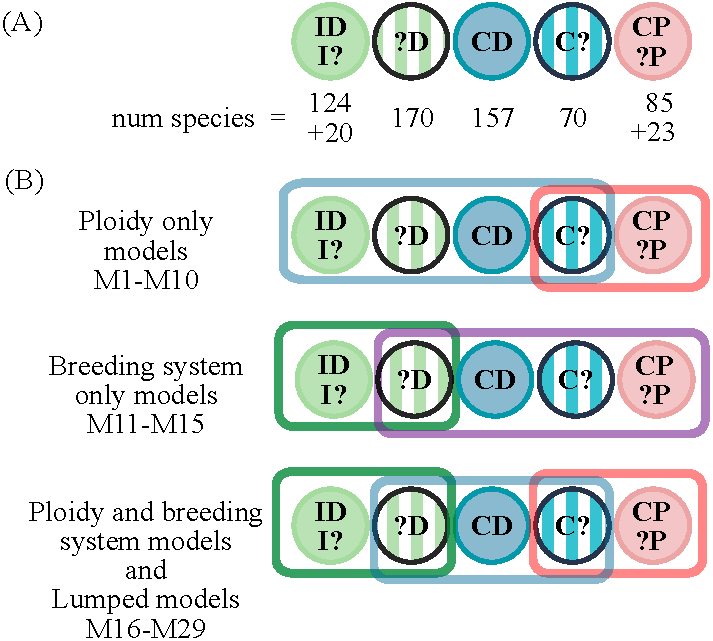
\includegraphics[width=0.5\textwidth]{states.pdf}
\caption{
Character states used for each of the models.
Each species retained on the tree belonged to one of five possible categories, depending on whether ploidy and/or breeding system were known.
The number of species in each is shown under the corresponding circles in the top row. % FIXME: Rosana, what are the numbers for CP and ?P ?
These categories were then grouped in a manner appropriate to the states of each model.
For example, there are 34 species that are self-compatible and of unknown ploidy; these are coded as either $D$ or $P$ in the D/P models (uncertain, or consistent with either state), as $C$ in the I/C models, and as either $CD$ or $CP$ in the ID/CD/CP models.
In all cases, species were coded as either $A$ or $B$ in the hidden state models.
The models depicted in the different rows use state spaces that are not comparable with one another.
For example, we cannot test whether the D/P model fits better than the I/C model because they use states that are not the same and are not `lumpable' \citep{tarasov_2019}.
%B: Hmmm. The presentation is economical, true, and I think it is retrospectively clear, and valuable, now that I've been thinking about the paper for a while. But it will be very difficult as a source of clarity for someone reading the paper the first time. The top graphical layout also implicitly communicates the idea that all "I" species must be "D", and that all "P" species must be also "C", which is not intuited easily. (Are they encoded like that?) Moreover, it's not made clear that the 'species' in question are, in fact, often polymorphic, which makes DPIC possible. The subsequent models require a bit of thought, which is not too bad, but the treatment of the state coding and specifically the sentence "In all cases, species were coded as either A or B in the hidden state models." is a bit terse for someone not familiar with HiSSE. 
}
\label{figure:stateclassifications}
\end{figure}


% R: I changed this models to go now in the new order

\begin{table}
\begin{tabular}{lcccccc} \toprule
% \begin{tabular}{@{}lcccccc@{}} \toprule
%\multicolumn{4}{r}{Models} \\ \cmidrule(r){3-5}
Model                        & Ploidy & Diploidization & Breeding  & Hidden & Num & Marginal \\
                             & &  &System & State & Parameters & Log-Likelihood \\ \midrule
1. D/P           &	Yes & 	No	& No	& No & 	5 &	-1193.66\\
2. D/P +$\delta$                      &	Yes  &	Yes &	No	&No	& 6	& -1182.93 \\
3. D/P+A/B        &	Yes & No &	No &	Yes &	10	&-1150.99\\
4. D/P+$\delta$+A/B                   &	Yes &	Yes	&No &	Yes &	11 &	\textbf{-1145.69}\\
5. I/C                       &	No & No	&Yes &	No &	 5 &  -1194.80 \\
6. I/C+A/B                   &	No &	 No	&Yes &	Yes	& 10 & \textbf{-1155.37}\\
7. ID/CD/CP      &	Yes & 	No &	Yes	&No &	9 &-1345.87\\
8. ID/CD/CP +$\delta$                 &	Yes & 	Yes &	Yes &	No &	10 & -1344.50\\
9. ID/CD/CP+A/B  & Yes & 	No	&Yes &	Yes	&15 &-1303.55 \\ 
10. ID/CD/CP+$\delta$+A/B              &	Yes 	&Yes &	Yes &	Yes &	16 & \textbf{-1300.35} \\
\bottomrule
\end{tabular}
\caption{
    The ten models and their marginal likelihoods.
    Values in bold are for the best models within each class that are comparable (see \cref{table:bayesfactors}).
    Abbreviations are D: diploid, P: polyploid, I: self-incompatible, C: self-compatible, A: one state of hidden trait, B: other state of hidden trait, $\delta$: diploidization.}
\label{table:marginallike}
\end{table}

\begin{table}
\addtolength{\tabcolsep}{-3pt}
\begin{tabular}{|c|c|c|}
\toprule
Ploidy Models & Breeding System Models & Ploidy and Breeding System Models \\ \midrule
{\begin{tabular}{lcccc}
 & 1 & 2 & 3 & 4 \\
1. D/P & $\cdot$	 &10.72 &	-37.24	&-31.94\\
2. D/P no $\delta$ &$\cdot$&$\cdot$ &	-47.97	&-42.66\\
\textbf{3. D/P+A/B}  &$\cdot$  & $\cdot$&	$\cdot$	& 5.30 \\
4. D/P+A/B no $\delta$ &$\cdot$& $\cdot$ & $\cdot$&$\cdot$ \\
\end{tabular}
}  & 
{\begin{tabular}{lcc}
 & 5 & 6\\
5. I/C &$\cdot$ & -39.43 \\
\textbf{6. I/C+A/B} &$\cdot$& $\cdot$ \\
& & \\
& & \\
\end{tabular}
} & 
{\begin{tabular}{lcccc}
& 7 & 8 & 9 & 10\\
7. ID/CD/CP & $\cdot$	&1.36 & -44.15&-40.95 \\
8. ID/CD/CP no $\delta$ & $\cdot$ & $\cdot$ & -45.51 &-42.31 \\
\textbf{9. ID/CD/CP+A/B}& $\cdot$ & $\cdot$ &$\cdot$	& 3.2 \\ 
10. ID/P/CD no $\delta$-A/B & $\cdot$& $\cdot$&$\cdot$ & $\cdot$\\
\end{tabular}
}\\
\bottomrule
\end{tabular}
% E: We will probably have to change the layout here because it's not technically a table.  But good enough for now.
\caption{
    Bayes factors for model comparisons.
    Each of the three boxes contains models that can be compared with one another, based on the character states they include (see \cref{figure:stateclassifications}).
    Models are numbered in as \cref{table:marginallike}.
    Bayes factors are reported on the natural log scale, so numbers greater than $+2$ mean that the model in the row label has `positive' support relative to the model in the column label; numbers less than $-2$ mean that model in the column label is the preferred one.
    Conventional thresholds for `strong' and `very strong' support are 6 and 10, respectively.
    The best model in each set is written in bold.
    In each case, it is the most complex model of the set.
}
\label{table:bayesfactors}
\end{table}



%\begin{tabular}{@{}lcccccccccc@{}} \toprule
%\multicolumn{4}{r}{Models} \\ \cmidrule(r){3-5}
%Model& 1& 2 & 3 & 4  &5 & 6& 7 & 8 & 9 & 10 \\
%Polyploidy & & & & & & & & & \\
%1. D/P &	-  &	10.727 &	-37.243	&-31.941& -	& - & - & - & - &- \\
%2. D/P no $\delta$ & -  & -  &	-47.97	&-42.668& -	& - & - & - & - &- \\
%3. D/P- A/B  & -  & -  &	-	& 5.302 & -	& - & - & - & - &- \\
%4. D/P no $\delta$-A/B &
%Breeding System& & & & & & & & & \\
%5. C/I & -  & -  &	-	& - & -	& -39.434 & - & - & - &- \\
%6. I/C-A/B &
%Polyploidy and Breeding System & & & & & & & & & \\
%7. CD/P/ID & -  & -  &	-	& - & -	& - & - &1.368 & -44.151&-40.951 \\
%8. CD/P/ID no $\delta$& -  & -  &	-	& - & -	& - & - &-& -45.519&-42.319 \\
%9. CD/P/ID-A/B& -  & -  &	-	& - & -	& - & - &-& -& 3.2 \\ 
%10.ID/P/CD no $\delta$-A/B &
%\bottomrule
%\end{tabular}

% E: Could we include a figure of the traits on the tree?  At least as supp info. TODO

\section{Results}
\subsection{Polyploidy and Diversification Models}
Similarly to the results obtained by \citet{mayrose_2011} and \citet{mayrose_2015}, we found that in the D/P polyploidy model the net diversification of diploids is larger than the the net diversification of polyploids since the net diversification distributions do not overlap (Figure 2(A)). This result holds true whether or not the diploidization parameter is present. However in the presence of  the diploidization parameter the net diversification rate of polyploids is nonnegative with probability 1 (Figure 2(A)), whereas in the absence of diploidization the net diversification rate of polyploids can be negative with a probability (HERE verify the quantile) (FIGURE 3(A)). In terms of the relative extinction, when the diploidization parameter is present both polyploids and diploids have posterior distributions that overlap, but that pattern changes in the absence of the diploidization parameter leading to a significant difference between relative extinction where polyploids have a significant higher relative extinction rate (see Supplementary Information).\newline

For the D/P- A/B model with diploididization the diploid and polyploid net diversification rates are overlapping for both state A and B of the hidden trait (Figure 2(B)). In this model, the differences in net diversification are due to the presence of a hidden trait and not to the differences in ploidy. When diploidization parameter is absent the hidden state is still driving the differences in diversification rates (Figure 3(B)).

\subsection{Breeding System and Diversification models }
In the I/C breedyng system model we found that the net diversification rate for self-incompatible state is larger than the net diversification rate for self-compatible state (Figure 2(C)). The net diversification rate for self-compatible has a probability distribution centered at zero.  \newline

When a hidden state is added in the I/C-A/B model, we found that under the hidden state A the self-compatible and self-incompatible net diversification rates are different. Under the hidden state B, those two rates overlap with a probability (HERE CALCULATE THAT) meaning that they are different with probability  (CALCULATE) (Figure 2(D)). These results agree with previous results found by  \citet{goldberg_2012}. However, \citet{goldberg_2012} used a ClaSSE  approach since they were interested in anagenetic and cladogenetic changes for self-incompatibility using a smaller subset of the data presented in the current work.

% Describe rate q_IC and hidden state rate

\subsection{Polyploidy and Breeding Sytem models}
In the ID/P/CD model we found that self-incompatible and diploid state has a significantly larger net diversification rate compare to both self-compatible diploid and polyploid rates. Meanwhile, both self-compatible diploid and polyploid posterior distributions of net diversification rates completely overlap (Figure 2(E)). When hidden state was added in the ID/P/CD-A/B model, we observed significant differences between self-compatible and self-incompatible diploids for both A and B values of the hidden state. Self-incompatible state had a larger net diversification rate than self compatible for both A and B states. However, the posterior distribution for the net diversification rate of polyploids overlaps with both the self-compatible and self-incompatible posterior distributions for each value of the hidden state(Figure 2F) meaning that polyploidy state is not significantly different from diploid in net diversification terms.  The resulting effect of adding the hidden state values is significant 


\subsection{Diploidization as an exploratory hypothesis}
In the D/P model  the diploidization rate $\delta$ and polyploidization rate $\rho$ are different from zero with probability 1. Diploidization rate is more uncertain than polyploidization. For the D/P no $\delta$ model, the polyploidization rate is still different from zero but has a wider 95\% credible interval (see Supplementary Information). In the D/P-A/B model the diploidization rate remains positive but there rate of polyploidization becomes really uncertain. Whereas, in the absence of diploidzation (D/P no $\delta$ A/B) the rate of polyploidy has a small credible interval \newline

For the model ID/P/CD containing both polyploidy and breeding system traits, we found that the diploidization rate is really uncertain with a MAP that is (CALCULATE VALUE HERE- close to zero). The polyploidization rate from self-incompatible diploid $\rho_I$ is slightly faster than the polyploidization rate from self-compatible diploid $\rho_C$  and that pattern remains the same for the ID/P no $\delta$/CD model(see supplementary information).
%Here I'm missing the MuHiSSE plots.

\subsection{Model selection}

In \cref{table:marginallike} we list the marginal likelihood in log scale for each of the models tested. In the table we show what are the different components included and excluded for each model as a a summary of the diagrams from \cref{figure:netdivall}. From the marginal likelihoods in log scale, the Bayes factors in log-scale were calculated as shown in table \cref{table:bayesfactors}. After testing every single pair of polyploidy modes (1-4) we found overwhelming evidence that the best polyploidy model is always  the D/P-A/B, that is the model with hidden state and diploidization. \newline
For the two models following the evolution of breeding system, the I/C-A/B is the best choice between models 3 and 4.\newline
The models that follow the diversification linked to both polyploidy and breeding system are the last 4 (models 5-8). When comparing using Bayes factores every two models we found that the IC/P/CD-A/B is always preferred over the rest, meaning that the model that has a hidden state and diploidization is chosen over the ones that lack either of both of those options.\newline
Therefore, the models that were chosen were always the ones containing a hidden trait, and in the case of polyploidy models, the ones containing a diploidization parameter $\delta$ are preferable.



Example in \cref{suppfigure:example}. % XXX

\begin{figure}
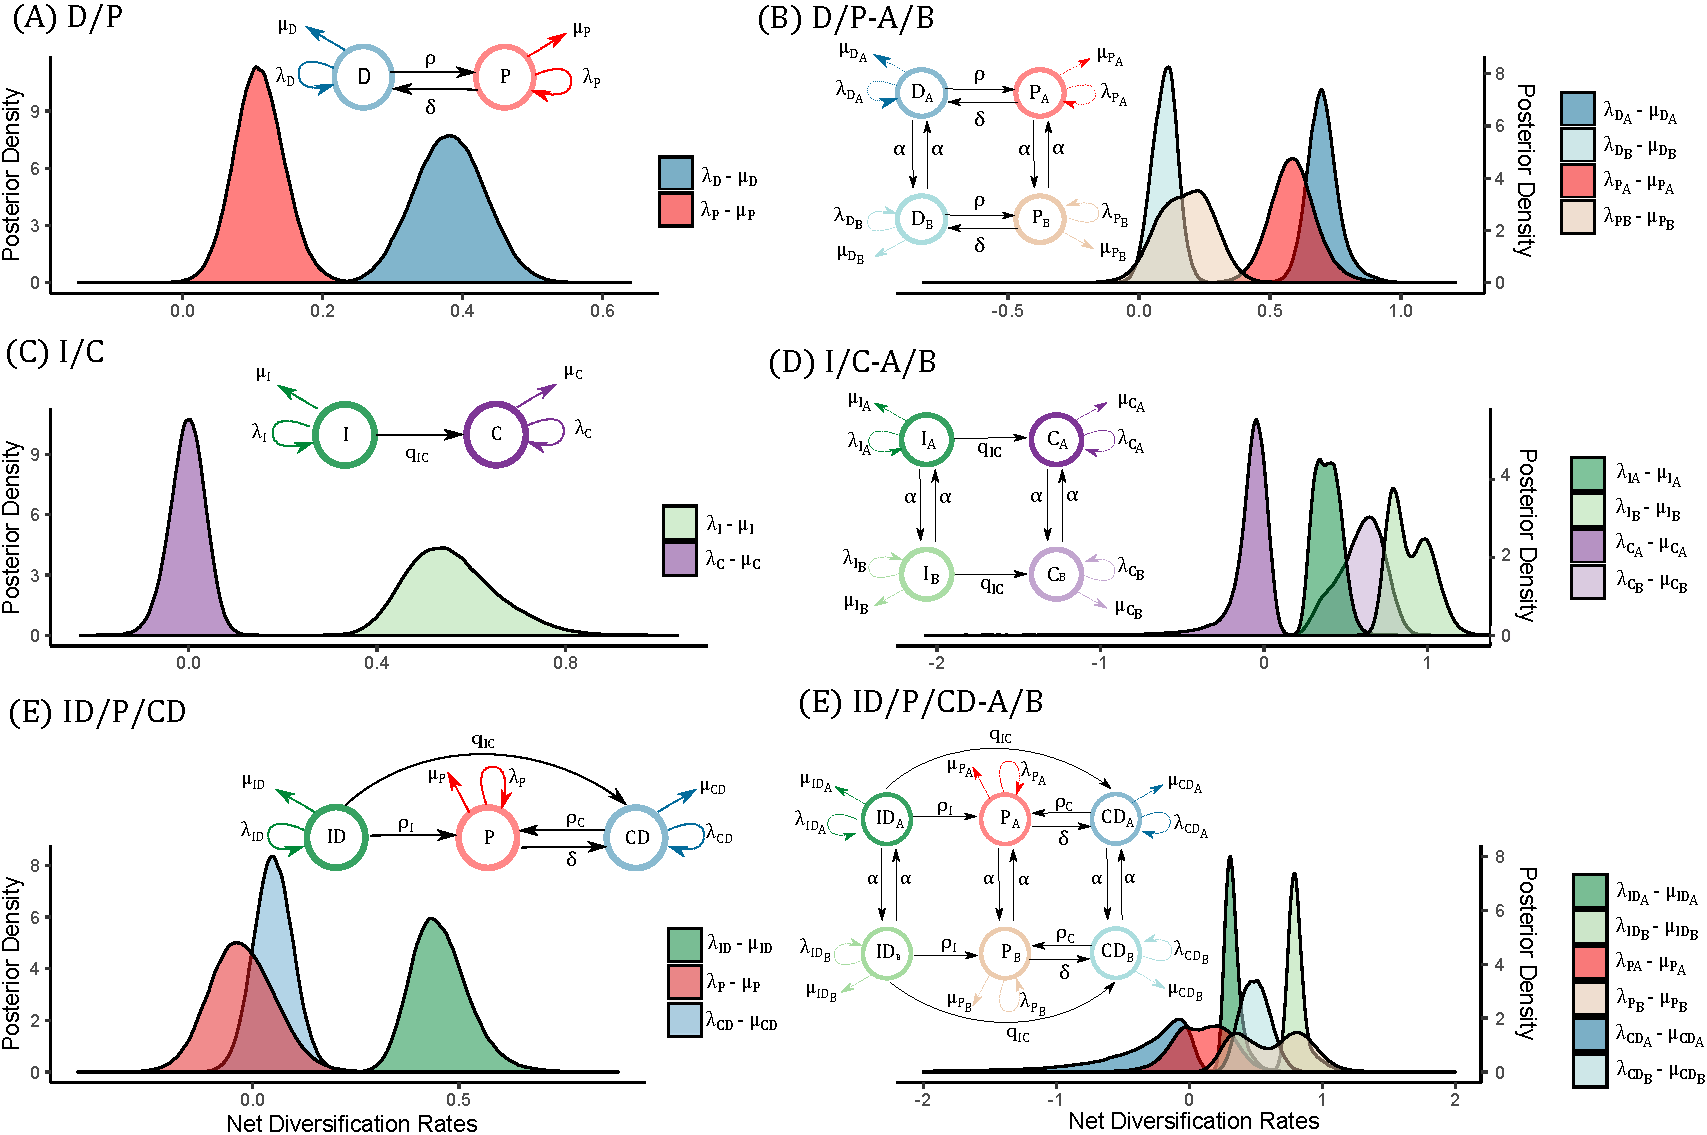
\includegraphics[width=\textwidth]{Netdiversificationallmodels.pdf}
  \caption{Net diversification rates for all models that include diploidization.}  
\label{figure:netdivall}
\end{figure}

\begin{suppfigure}
\caption{example Supp Info figure} % XXX
\label{suppfigure:example}
\end{suppfigure}

\section{Discussion}

% outline
% - disentangling effects
% - general value of approach
%  		another kind of confounding processes, not only transition and diversification, but "other diversifications" and "other transitions", esp. correlated
%
% - our study key findings and details
% - effects of Ploidy (as %R)
% - trumped by BS
% - no difference on background of SC 
% - discuss data/models and their long/shortcomings: ClaSSE, will's idea for stochastic mapping
% - how to improve / what next
%  (may be useful to study in SC families)
%
% - pathways
% 
%- diploidization
% - rate, effect
% - history in solanaceae
%
% - summary


We investigated the individual and joint effects of ploidy and breeding system states in diversification of Solanaceae.
Most significantly, we found that the effects of ploidy, inferred as significant when it is the only trait under consideration, are trumped by breeding systems when the two traits are considered jointly.
Interestingly, the difference in diversification rates between the diploids and polyploids is negligible on the background of self-compatibility.
%B: should we mention here that the hidden states presage these results in each case? Maybe we don't want to make too much of that, but it is fairly interesting. Also possibly hit that in your paragraph(s), below.
In the same vein, the difference in diversification rates between self-incompatible and self-compatible lineages is smaller in the diploid genomic background.
In our final analyses, motivated by the widespread findings of paleopolyploid ancestry across angiosperms, we did not recover strong support for inclusion of diploidization process.
Below, we discuss the key findings, and outline a broad strategy for applying phylogenetic comparative methods in the study of complex interactions among traits, in the context of diversification.
%  Surprising outcomes: (1)  D and P on background of C, and (2) SC not as dead of an end as it was in goldberg2010, if P is partitioned out (can be framed as kind of path-dependence, i.e. qIC path different than rho path, or same as (1), so that I and C are less different on the background of D.


% - value of approach
Disentangling the patterns of diversification linked to  multiple traits allowed us the opportunity to model and test complex hypotheses about the heterogenous diversification process in Solanaceae.
Species are created and go extinct based on multiple and often highly correlated phenotypes. However, estimating the speciation and extinction rates remains challenging. Estimating rates of trait linked diversification models is not only a problem of difficult parametric inference (as disscussed in  \citet{rabosky_2010, beaulieu_2015}),but also, a problem of inadequate model specification that can result in misleading inferences when the presence of a second trait has a complex interaction with the focus trait first used to model diversification. We presented a roadmap with a series of analyses that can help scientists to identify if an unknown or unobservable trait is worth pursuing. By carefully aggregating and curating ploidy and breeding system data for Solanaceae, we showed how  the complex interaction between ploidy and breeding system  can lead to diversification conclusions that differ from the diversification conclusions of models that focus on one trait at a time.

% - what happens if PD only, Hidden states
Previous analyses of polyploidy linked to diversification showed how diploids had greater net diversification rates than polyploids when exploring across multiple clades of the angiosperm phylogeny \citet{mayrose_2011, mayrose_2015}. 
Using the most complete dataset for ploidy in a phylogenetic tree for Solanaceae, we were able to replicate the results found by \citet{mayrose_2011} where polyploids have a slower net diversification compare to diploids.
However, we expanded this study to accommodate  background heterogeneity in the diversification process.
When adding heterogeneity we found that it was more likely that an unobserved trait linked to diploid state was the one leading the net diversification patterns, and that there were some ``second-class"  diploids that were not different from  polyploids  in diversification terms (Figure 2A).
This result made us question whether there was a second trait linked to diploidy that could make a differential in the diversification progress.

%     main finding about our traits
For Solanaceae, looking into self-incompatibility was a logical step.
Previous studies have shown that self-incompatible Solanaceae species have also higher rates of diversification compared to their self-compatible counterparts \citep{goldberg_2012}. 
Again, in our sample when looking only into breeding system linked to the diversification process we were able to replicate the slower net diversification for self-compatible taxa (Figure 2C). When this model was expanded to incorporate hidden states we found again that some self-incompatible taxa have faster net diversification rates than self-compatible taxa. However, there is again a  different class of taxa where those differences are not as striking (Figure 2D).  However, investigating both  both polyploidy and breeding system simultaneously for every species in our sample, allowed us to further investigate why some diploids were quantitatively different than polyploids, or why some self-incompatible taxa would be different in diversification terms from some self-compatible when a second class is not.
In the three-state diversification model ID/CD/CP, we represented the complex interactions between ploidy and breeding system. We found that self-incompatible diploids have faster and positive rates than self-compatible diploids and polyploids, and that the difference between the  rates of net diversification of self-compatible diploids is not as large (Figure 2E) as first found by binary trait diversification models (Figure 2A).
This result is key, it not only aligned with the net diversification results from the D/P+A/B model, where a `	`hidden-trait" seem to be dictating the diversification pattern but it also aligned with the hidden state model I/C+A/B where some class of self-compatible net diversification rate might be overlapping with two net diversification rates of self-incompatible.
% Removed by R. Therefore, we consider that finding a heterogenous result in the hidden trait approaches should be be treated as evidence of a second trait that is necessary to consider.
% Removed by R. Pursuing knowledge of  such trait can result on a clearer picture of the importance of trait linked diversification patterns, but also on a better reconstruction on past events in phylogenies.

%     more generally, not okay to approximate musse with bisse when states are correlated (cf Pyron)

% alpha is always low
%     new supp fig showing how A & B are inferred on the tree?  at least for ID/CD/CP+A/B model
%     maybe we can hypothesize factors that underlie the hidden state (geography?)

% pathways: compare/contrast with robertson2011
%     \rho_I > \rho_C in all!

% Will: I really like the pathways analyses and have a couple comments
%
% 1) Were the "without diversification" and "with diversification" analyses computed
%    using the same MAP transition rate estimates? Transition rates among states will
%    be very different if estimated using a model that is diversification-independent 
%    compared to when estimated with a trait-dependent diversification model. Since the point of 
%    showing these side-by-side seems to be emphasizing the importance of considering trait-dependent
%    diversification, I wonder how different the "without diversification" contributions would be
%    if calculated from transition rates estimated using a diversification-independent model.
%  R- Good point. Emma will clarify
%
% 2) I think stochastic mapping would be another useful perspective on the pathways question
%    (and yeah, its a bit late in the game to propose analyses, so maybe next time!). With stochastic 
%    mapping we could use the entire posterior estimate of the transition rates rather than a point
%    estimate. But more importantly we'd get the relative contributions of the pathways estimated 
%    over the actual Solanceae tree (which has a lot of short interdependent branches rather than 
%    hypothetical long branches). 
%R- It will, it was actually on my code I think for the ID/CD/CP I have the stochastic mapping trees. We can do it for the revision. I think the only model where it could not finish was the ID/CD/CP+A/B (was taking forever and we had the restriction of time from MSI)

% 3) I'll bet allowing cladogenetic transitions would make the one-step ID/CP even more dominant.
%    I added the paragraph below regarding cladogenetic transitions, but it doesn't really fit with
%    the rest of the discussion, so modify or discard as needed:
Our work shows that a diploid Solanaceae lineage is much more likely to take a
one-step ID/CP pathway to polyploidy rather than a two-step ID/CD/CP pathway. 
We modeled both of these pathways as anagenetic character changes occurring within a species.
However \citet{goldberg_2012} showed that I/C transitions are often associated with speciation events, and similarly \citet{freyman_2017} demonstrated that D/P transitions may also be associated with speciation events. 
Models that fail to consider transitions that occur at speciation (cladogenetic changes) may
make misleading estimates of anagenetic transition rates.
The HiSSE-based models introduced in our work here could be extended to incorporate cladogenetic transitions. 
It is possible that allowing for cladogenetic transitions may enable the one-step pathway
to even further dominate over the two-step pathway to polyploidy, but this remains to be tested in future work.

% And, are diversification rates of polyploid SC lineages different if one or other path was taken? \citet{charlesworth1985} % E: This is a great question.  We don't answer it with this round of analyses.  But discuss?

% where WGD is in Solanaceae--motivation and delta rate analyses
% diploidization: comment
Diploidization needs to be considered in diversification models because higher rates of net diversification (speciation minus extinction) in diploids can be obtained from models that ignore the possibility of a polyploid lineage that has diploidized being the diversification enhancer. Hence, in a diploidization lacking model, diploids will show higher rates of diversification when in fact it is a polyploidy event and its subsequent diploidization that generated higher speciation and less extinction.  By adding diploidization to models of polyploidy linked to diversification it is possible to recover this complicated scenario and to reconcile genomic evidence with stochastic models. In past studies by \citet{mayrose_2011, mayrose_2015} diploidization could not be formally  considered in models because ploidy classification was done via chromosome change models (i.e. Chromevol \citep{glick2014}) that do not allow for reversion of polyploidy. However, in our dataset ploidy was assigned based on data aggregated from independent studies (see supplementary information and citations in archived dataset) that come from field or cytogenetic studies. In the cases where ploidy level was assigned by us based chromosome multiplicity at the genus level, estimating diploidization  might be a potential issue due to ploidy misclassification.  

% B: This is my pitch for motivation of the \delta paragraph and/or wording for how to reconcile estimates and genomic data (providing summary of data--to date)
Diploidization is widely considered to be relatively rare, compared with polyploidization, but flowering plant lineages are thought to have experienced at least one round of polyploidization in their evolutionary history.
As a consequence, it is possible that nearly all extant species classified as ``diploid" in our analyses are possibly secondary diploids, having undergone both polyploidization and re-diploidization.
Genomic evidence indicates that such an event may have occurred prior to the origin of the family Solanaceae. 
\citet{ku2000} and \citet{blanc2004} posited that the lineage leading to tomato, \textit{Solanum lycopersicum}, may have experienced one or more paleopolyploid events.
A subsequent analysis of synteny between grape and \textit{Solanum} genomes, as well as the distribution between inferred paralogs within \textit{Solanum} (tomato and potato) genomes both suggest that this lineage experienced a likely round of ancient genome duplication or triplication \citep{tomato2012}. 
The age of the peak of paralog Ks distances, is approximately 71 million years \citep{tomato2012}. 
If this is the case, then all of the genomes may have been subsequently re-diploidized, because common base chromosome numbers this and related families are n=11-12. 

%Not unlikely, because Arabidopsis n=5.
On the other hand, studies comparing map-based genome synteny within the family find no evidence for recent polyploidization-diploidization \citep{wu_2010a}. 
Simple genome re-arrangements appear sufficient to explain chromosomal evolution between a number of species, including all of those in the relatively cytogenetically conserved `x=12' group, which includes tomato, potato, eggplant, pepper, and tobacco.
%B: Once this is re-arranged, and made to fit with the rest of the discussion, add what this has to do with re-diploidization and how to interpret $\delta$.
Therefore, it is not surprising that for all models diploidization  had wide credible intervals for parameter $\delta$. Despite the classification and genomic limitations to assign ploidy levels and diploidization, we found support for models that include pararmeter $\delta$, meaning that further studying this process is worth pursuing.

%     effect on inferred diversification


% generality of approach
%
% issues
%     meaning of diploidization parameter
%     irreversibility SI -> SC assumption

% Missing a good concluding paragraph.


%--------------------------------------------------
\section{Acknowledgements}
%--------------------------------------------------

NSF DEB-1655478.
The Minnesota Supercomputing Institute (MSI) at the University of Minnesota provided computing resources for this project.

%--------------------------------------------------
% References
%--------------------------------------------------

\clearpage

\setstretch{1}
\bibliography{refs}
\bibliographystyle{evolution} % E: remove URLs
\setstretch{\stretchby}

% E todo: add latex stuff to make supp info easier

\end{document}
